\section{Process, Thread, Syscalls}

% ======= Lecture 1 =========

The OS's solution to virtualization is \textit{limited direct execution},
with the key abstraction being the \textbf{process}. By direct execution, the
cpu is set so that the next instruction is fetched from the code of the process
to be executed, but with limited operations a process can perform. A process uses
\textbf{system calls} to do something privaleged.

During boot time, the OS fills the interrupt table, runs the ``main'' loop
(fetch instr, decode instr, execute instr, fetch instr, ...), and then an
interrupt occurs, forcing the CPU to change modes (disabling other interrupts),
register {\tt \%eax} contains the interrupt number, which is used ot set the PC
to the start of interrupt handler. \textit{efficient virtualization} by
catching illegal instructions (throws exception) and by periodic hardware
generated timer interrupts forcing OS control (context switches).

Through \textbf{bootstrapping}: hardware stores small program in non-volatile
memory which knows how to access some hardware, starts up in system mode, and
initializes OS data structres, the {\tt init} process, and switches to user
mode and waits.

The  \textbf{process} is an abstraction for execution, it has its own view of
memory and contains <address space: OS and program;execution stack, PC,
registers, OS resources, kernel execution, PID>. The \textbf{PCB} is where OS
data about a process is stored. The PCB contains <process state, PC, CPU regs,
CPU scheduling info, mem mgmnt info, accounting info, I/O info>

The OS uses \textbf{State Queues} (ready, running blocked) to represent state
of all processes. PCBs are enqueed to the queue that represents its state. Going
from {\tt Ready} to {\tt Running} involves a \textbf{context switch}. Exiting
involves freeing address space, closing files, etc, but retains its PID until
its parent cleans it up. {\tt fork() } creates a new process by initializing the
PCB, creating an address space (with a \textit{copy} of the parents address
space), and places the PCB on ready queue. {\tt int exec(char *prog, char **argv)}
starts a new program by stopping the current process, loading {\tt prog}, and
places the PCB onto the ready queue, but it does \textit{not} create a new
proceess, instead it loads {\tt prog} into the current process.

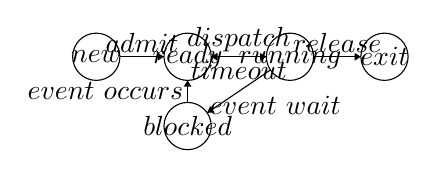
\begin{tikzpicture}[scale=0.1]
\tikzstyle{every node}+=[inner sep=0pt]
\draw [black] (9.2,-18.7) circle (3);
\draw (9.2,-18.7) node {$new$};
\draw [black] (20.8,-18.7) circle (3);
\draw (20.8,-18.7) node {$ready$};
\draw [black] (20.8,-27.5) circle (3);
\draw (20.8,-27.5) node {$blocked$};
\draw [black] (33.8,-18.7) circle (3);
\draw (33.8,-18.7) node {$running$};
\draw [black] (45.8,-18.7) circle (3);
\draw (45.8,-18.7) node {$exit$};
\draw [black] (12.2,-18.7) -- (17.8,-18.7);
\fill [black] (17.8,-18.7) -- (17,-18.2) -- (17,-19.2);
\draw (15,-18.2) node [above] {$admit$};
\draw [black] (23.8,-18.7) -- (30.8,-18.7);
\fill [black] (30.8,-18.7) -- (30,-18.2) -- (30,-19.2);
\draw (27.3,-18.2) node [above] {$dispatch$};
\draw [black] (30.8,-18.7) -- (23.8,-18.7);
\fill [black] (23.8,-18.7) -- (24.6,-19.2) -- (24.6,-18.2);
\draw (27.3,-19.2) node [below] {$timeout$};
\draw [black] (36.8,-18.7) -- (42.8,-18.7);
\fill [black] (42.8,-18.7) -- (42,-18.2) -- (42,-19.2);
\draw (39.8,-18.2) node [above] {$release$};
\draw [black] (31.32,-20.38) -- (23.28,-25.82);
\fill [black] (23.28,-25.82) -- (24.23,-25.78) -- (23.67,-24.96);
\draw (31.94,-23.6) node [below] {$event\mbox{ }wait$};
\draw [black] (20.8,-24.5) -- (20.8,-21.7);
\fill [black] (20.8,-21.7) -- (20.3,-22.5) -- (21.3,-22.5);
\draw (20.3,-23.1) node [left] {$event\mbox{ }occurs$};
\end{tikzpicture}
% ======= Lecture 2 =========


Programs and the OS communicate through \textit{system calls}. \textbf{interrupts} are used to keep apps from using recources w/o asking permission. When an
interrupt occurs, there must be a \textit{reason}, which is stored in a
register that is used to invoke a \textit{handler}. The result of a syscall
is stored in register {\tt EAX}.  
 A syscall dispatch: <kernel: give each syscall a num and put in
syscall table, user calls syscall n, hardware switches to kerne mode and
invokes an interrupt dispatch, looks up syscall num with table, invokes the
function, returns {\tt iret}>

\subsection*{Threads}
separating address space from execution allows for multiple executions in one
space. This allows for easy sharing data, easy creation/destruction, and
performance increases. \textbf{threads} get their own space in the stack and
their own PC, but share a heap. Kernel level threads may suffer from a lot of
overhead, since they still require system calls, and need to support all
languages, etc. So user level threads are used instead, without kernel
involvement. Limitations of user level threads are: <invisible to OS: OS can
make poor decisions regarding them, such as descheudling a thread w/ lock>.

